\documentclass[../../main.tex]{subfiles}

\begin{document}
    Bei der Magnetresonanztomographie (MRI - engl.: Magnetic resonance imaging) erzeugt man aus dem gemessenen FID ein räumliches Bild. Dazu wird ein Gradient im sonst idealerweise homogenen B-Feld in z-Richtung angelegt. Dieser Gradient sorgt für eine leichte Verschiebung der Larmorfrequenzen im Raum. Durch eine Fouriertransformation 
    \begin{align}
        \rho(x) = \int A(k) e^{-i2\pi k\cdot x}dk
    \end{align}
    erhält man eine ortsabhängige Funktion des gemessenen Signals.
    
    \subsubsection{1D - MRI}
        Im folgenden Teil wird eine Flasche mit zwei getrennten, rohrförmigen Kammern untersucht. Beide Kammern sind mit Wasser gefüllt. In der einen Kammer ist ein unbekanntes Salz im Wasser gelöst. Dies lässt ein unterschiedliches Ansprechen beider Substanzen auf die Polarisationsdauer und die Phasengradientendauer vermuten. Dieser Zussammenhang wird im nächsten Abschnitt mittels einer 2D-MRI untersucht. In diesem Teil steht die räumliche Ausdehnung des Körpers im Fokus, die in alle drei Raumrichtungen erfasst werden soll. Für die Durchführung wurden die optimierten Shimming-Einstellungen aus den vorherigen Versuchsteilen verwendet. Die Polarisationsdauer beträgt \SI{4000}{\milli \second}, die Phasengradientendauer \SI{100}{\milli \second} und die Echozeit \SI{200}{\milli \second}. Gemessen wurde über eine Länge von \SI{200}{\milli \metre}. Es wurden insgesamt drei Messungen, einmal in x-,y- und z-Richtung durchgeführt. Dabei ist die x-Richtung, die Achse entlang der Spule, die z-Richtung, die Richtung des Erdmagnetfeldes und die y-Richtung die Richtung der Normale der x-z-Ebene.
        \begin{figure}[h!]
            \begin{subfigure}[c]{0.5\textwidth}
                \includegraphics[width=\linewidth]{Bilddateien/12/X/Fig_1}
                \subcaption{x-Richtung}
                \label{fig:MRI_1D_X}
            \end{subfigure}
            \begin{subfigure}[c]{0.5\textwidth}
                \includegraphics[width=\linewidth]{Bilddateien/12/Y/Fig_1}
                \subcaption{y-Richtung}
                \label{fig:MRI_1D_Y}
            \end{subfigure}
            \begin{subfigure}[c]{0.5\textwidth}
                \includegraphics[width=\linewidth]{Bilddateien/12/Z/Fig_1}
                \subcaption{z-Richtung}
                \label{fig:MRI_1D_Z}
            \end{subfigure}
            \caption{Abmessungen der Flasche mit zwei Kammern in x-, y- und z-Richtung.}
            \label{fig:MRI_1D}
        \end{figure} 
        In Abb. \ref{fig:MRI_1D} sind die Kurven der Fouriertransformation aus den gemessenen Werten dargestellt. Die Messung wurde mit einer Bandbreite von \SI{64}{\hertz} durchgeführt. Da über \SI{200}{\milli \metre} gemessen wird, können die x-Achsen mit dem Faktor \SI{3,125}{\milli \metre \per \hertz} umgerechnet werden. Aus der Messung in x-Richtung, also entlang der Spulenachse, ist zu erkennen, dass die Röhren in der Flasche ca. \SI{100 +- 20}{\milli \metre} lang sein müssen. Aus der Messung in y-Richtung geht eine Breite des Röhren von \SI{50 +- 10}{\milli \metre} hervor. Diese Messung ist vermutlich dadurch verfälscht, dass die zwei Röhren hier leicht versetzt hintereinander liegen. Die Messung in Z-Richtung ist aus diesem Zusammenhang heraus, die Bessere, da hier beide Peaks für je eine Röhre gut zu sehen sind. Aus dieser Messung geht für beide Röhren eine breite von \SI{34,4 +- 5}{\milli \metre} hervor. Die durchgeführte Messung kann als Mittelung der Resonanzen auf einer Ebene verstanden werden. Dabei ist der Vektor der gemessenen Achse der Normalenvektor dieser \glqq{}Mittelungsebene\grqq{}. Da die Probe zwischen den Messungen nicht bewegt worden ist, müssen die Integrale der Peaks in x-,y- und z-Richtung denselben Wert besitzen. Die ermittelten Werte sind in Tabelle \ref{tab:MRI_1D_Integrale} dargestellt. Sie stimmen im Rahmen der Unsicherheiten miteinander überein.
        \begin{table}[h!]
            \centering
            \begin{tabular}{r|c}
            Richtung & Peakintegral                            \\ \hline
            x        & $\SI{286 +- 14}{\milli \metre \second}$ \\
            y        & $\SI{269 +- 13}{\milli \metre \second}$ \\
            z        & $\SI{279 +- 14}{\milli \metre \second}$
            \end{tabular}
            \caption{Integrale der Peaks aus den 1D-MRI-Messungen.}
            \label{tab:MRI_1D_Integrale}
        \end{table}
        
    \subsubsection{2D - MRI}
        Beim 2D-MRI wird durch mehrere 1D-Messungen in zwei Richtungen ein zweidimensionales Bild erzeugt. Ziel dieser Messung ist, die Röhre mit den im Wasser gelösten Ionen zu finden. Theoretisch wäre dies aufgrund der guten Lage der Röhrchen bei der 1D-MRI in z-Richtung auch möglich gewesen. Aus den vorherigen Versuchsteilen ist bekannt, dass die Anregung der gelösten Ionen im Wasser schon bei kleineren Polarisationsdauern stark wird. Das wird in diesem Versuchsteil genutzt, um die Röhre mit den gelösten Ionen von der ohne Ionen zu unterscheiden. Bei kleinen Polarisationsdauern ist die Anregung des reinen Wassers so klein, dass dieses kaum zu sehen ist. 
        \begin{figure}[h!]
            \begin{subfigure}[c]{0.5\textwidth}
                \includegraphics[width=\linewidth]{Bilddateien/13/YZ-4000-100/Fig_1}
                \subcaption{$t_{pol} = \SI{4000}{\milli \second}$ und $t_{pg} = \SI{100}{\milli \second}$}
                \label{fig:MRI_2D_YZ_4000_100}
            \end{subfigure}
            \begin{subfigure}[c]{0.5\textwidth}
                \includegraphics[width=\linewidth]{Bilddateien/13/YZ-500-100/Fig_1}
                \subcaption{$t_{pol} = \SI{500}{\milli \second}$ und $t_{pg} = \SI{100}{\milli \second}$}
                \label{fig:MRI_2D_YZ_500_100}
            \end{subfigure}
            \begin{subfigure}[c]{0.5\textwidth}
                \includegraphics[width=\linewidth]{Bilddateien/13/YZ-500-50/Fig_1}
                \subcaption{$t_{pol} = \SI{500}{\milli \second}$ und $t_{pg} = \SI{50}{\milli \second}$}
                \label{fig:MRI_2D_YZ_500_50}
            \end{subfigure}
            \begin{subfigure}[c]{0.5\textwidth}
                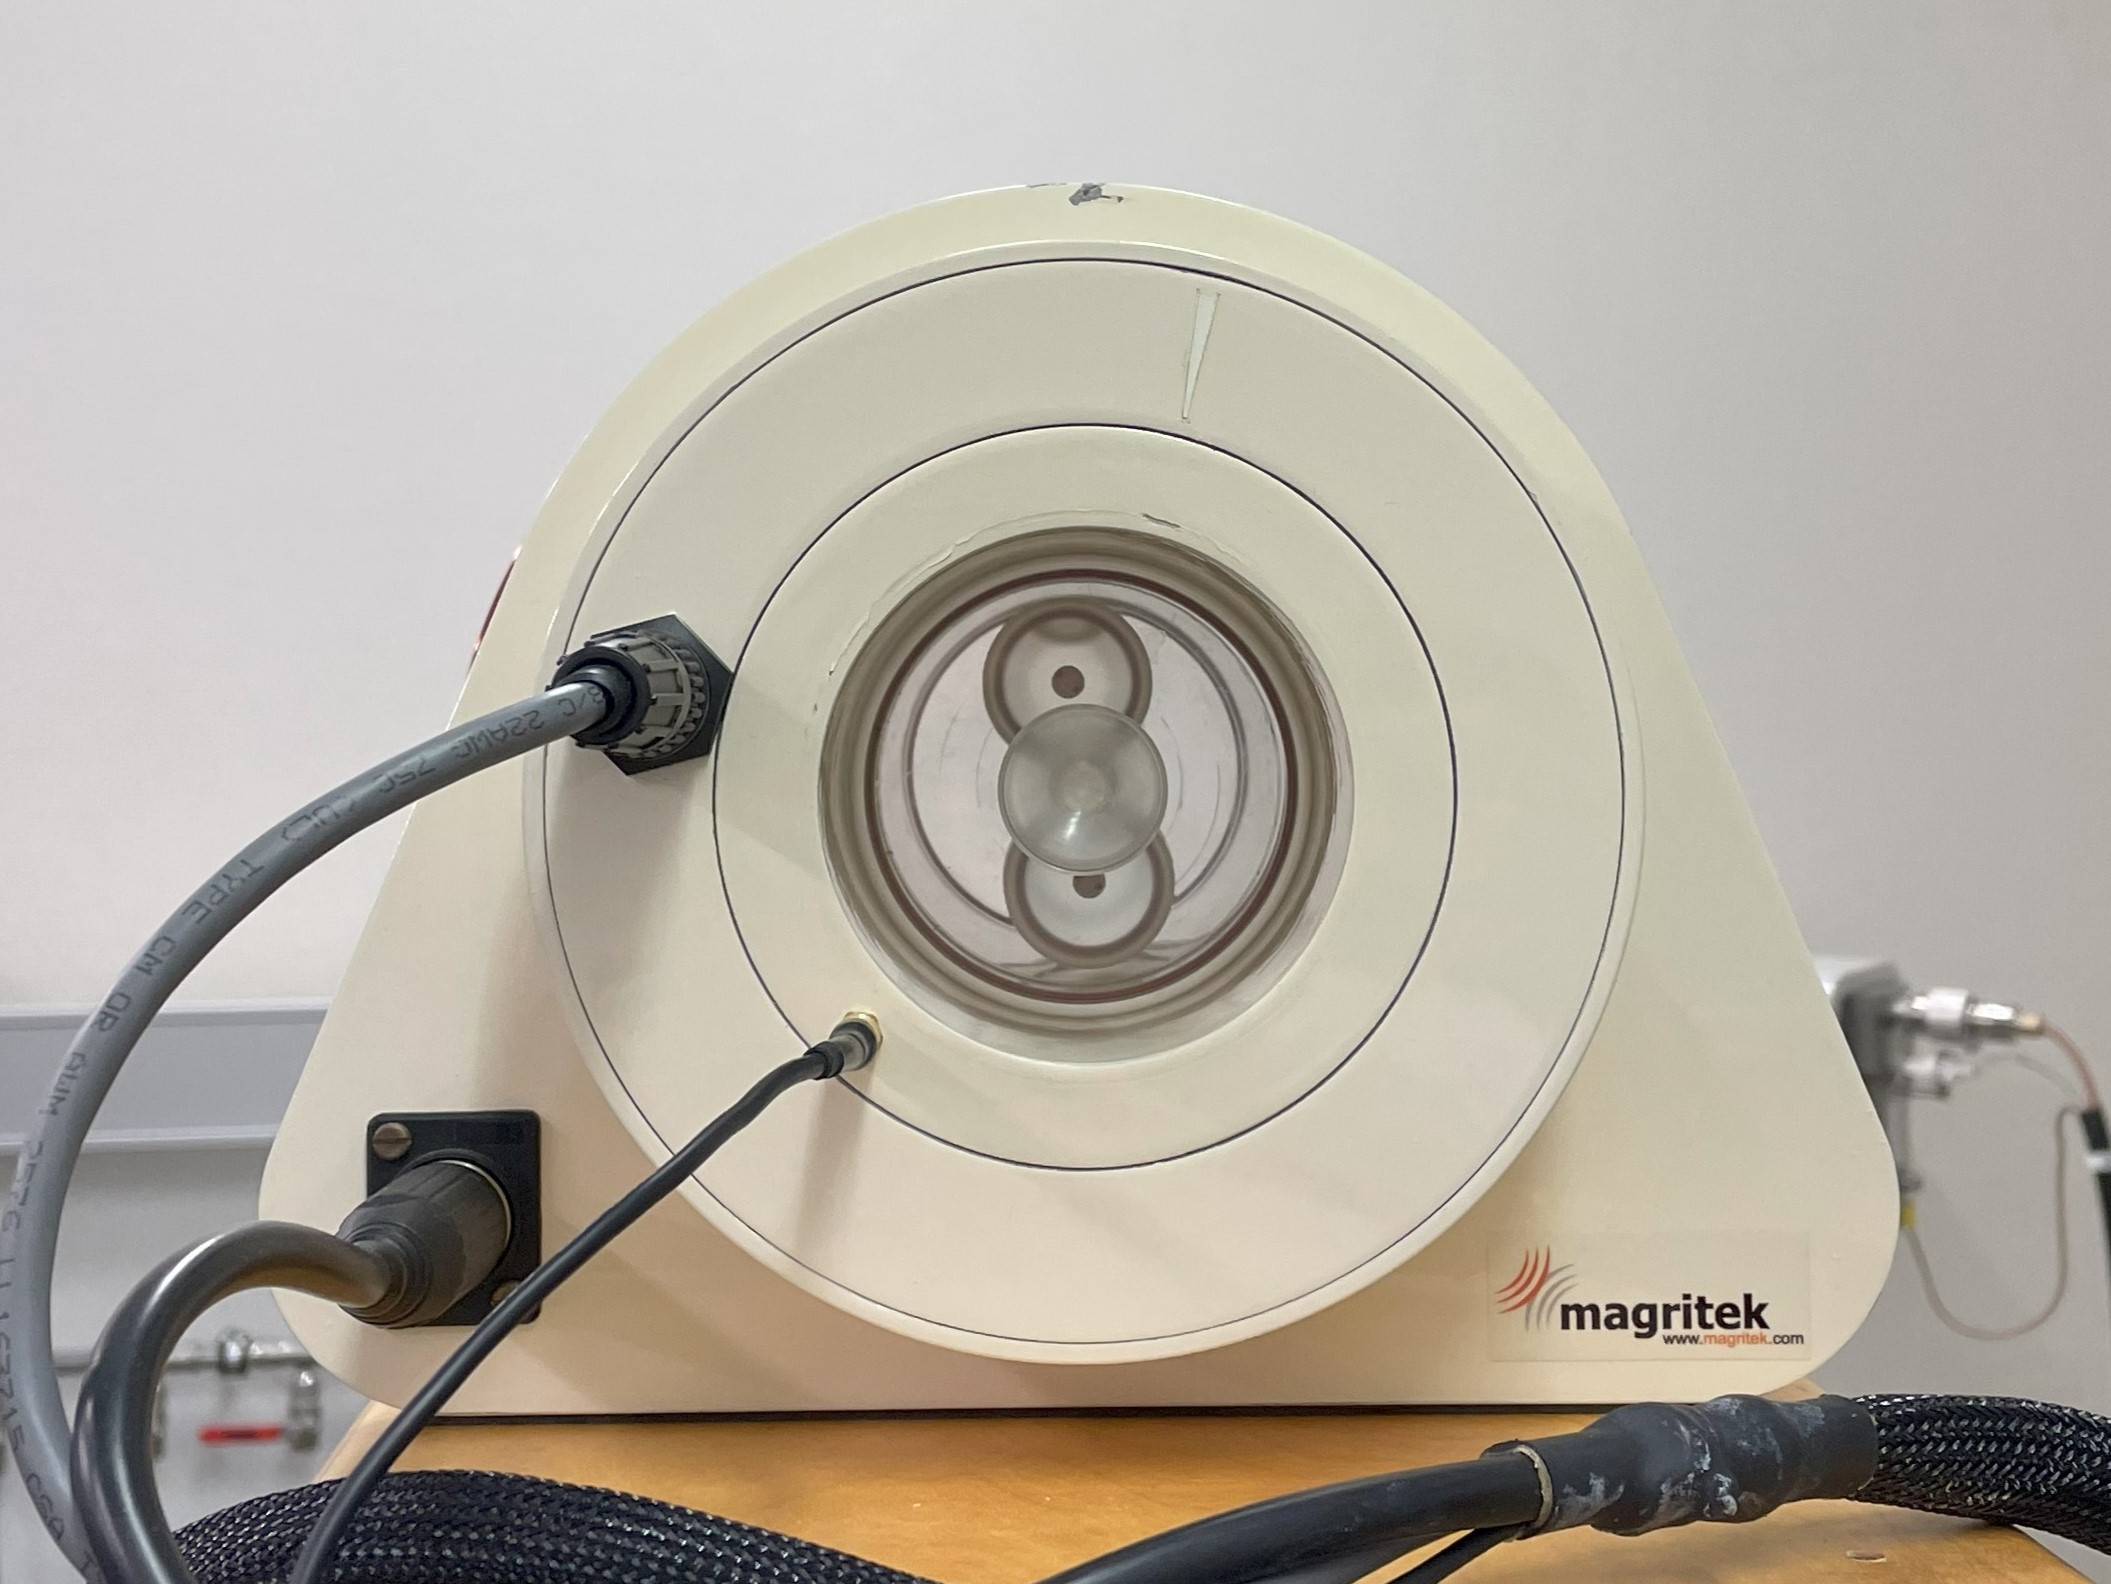
\includegraphics[width=\linewidth]{Bilddateien/13/MRI_Phantom_crop.jpg}
                \subcaption{Lage der Probe in der Spule}
                \label{fig:MRI_2D_Phantom}
            \end{subfigure}
            \caption{MRI-Bilder mit unterschiedlicher Polarisationsdauer $t_{pol}$ und Phasengradientendauer $t_{pg}$. Die Amplituden des fouriertransformierten Messsignals sind mit einer Farbskala dargestellt. Als Referenz ist unten rechts die Lage der Probe in der Spule abgebildet.}
            \label{fig:MRI_2D}
        \end{figure}
        Die Ergebnisse der 2D-MRI-Messung sind in Abb. \ref{fig:MRI_2D} dargestellt. Gemessen wurde mit einem Sichtfeld (field of view) von \SI{100}{\milli \metre} x \SI{100}{\milli \metre}. Der Einfluss der Polarisationsdauer $t_{pol}$ ist gut zu erkennen. Die Reduktion der Polarisationsdauer zwischen Abb. \ref{fig:MRI_2D_YZ_4000_100} und \ref{fig:MRI_2D_YZ_500_100} sorgt für eine Abschwächung der Amplitude. Auffallend ist, dass die Amplitude des unteren Peaks stärker abfällt, als die des oberen Peaks. Das entspricht genau der Erwartung aus dem Versuchsteil mit dem im Wasser gelösten Manganchlorid. Die Resonanz bei der Probe mit dem gelösten Salz nimmt langsamer ab, als in der Probe ohne gelöstes Salz. Zwischen den Messungen aus den Abb. \ref{fig:MRI_2D_YZ_500_100} und \ref{fig:MRI_2D_YZ_500_50} wurde die Phasengradientendauer reduziert. Die Amplitude im oberen Peak wird wieder etwas größer, während das Hintergrundrauschen abnimmt. Mit den vorliegenden Daten lässt sich ermitteln, dass in der oberen Röhre wohl Ionen gelöst sind. 
\end{document}